\section{Sensibility Testbed Design}\label{sec-design}

This section describes the design of the Sensibility Testbed. 
%On one hand, Sensibility Testbed manages how device owners make their
%devices accessible to the research community. On the other hand,
%it offers technical resources to researchers that allow them to
%securely collect data from remote mobile devices. 
We start with
an overview of the testbed infrastructure (Section~\ref{sec-overview}), 
and description of each testbed component 
(Section~\ref{sec-component}), then finally discuss the default policies 
of Sensibility Testbed that are used to protect device owners' personal 
information (Section~\ref{sec-irb-policies}).


\subsection{Overview}\label{sec-overview}

%\subsubsection{Interacting Parties}\label{sec-parties}
In Sensibility Testbed, there are three types of interacting
parties, as shown in Figure~\ref{fig-arch}: mobile \textit{devices} 
owned by ordinary people, with our app installed; a 
\textit{clearinghouse} server that discovers and configures
participating devices; and \textit{experimenters} who want to run
experiments on mobile devices. 

\begin{figure}
\center{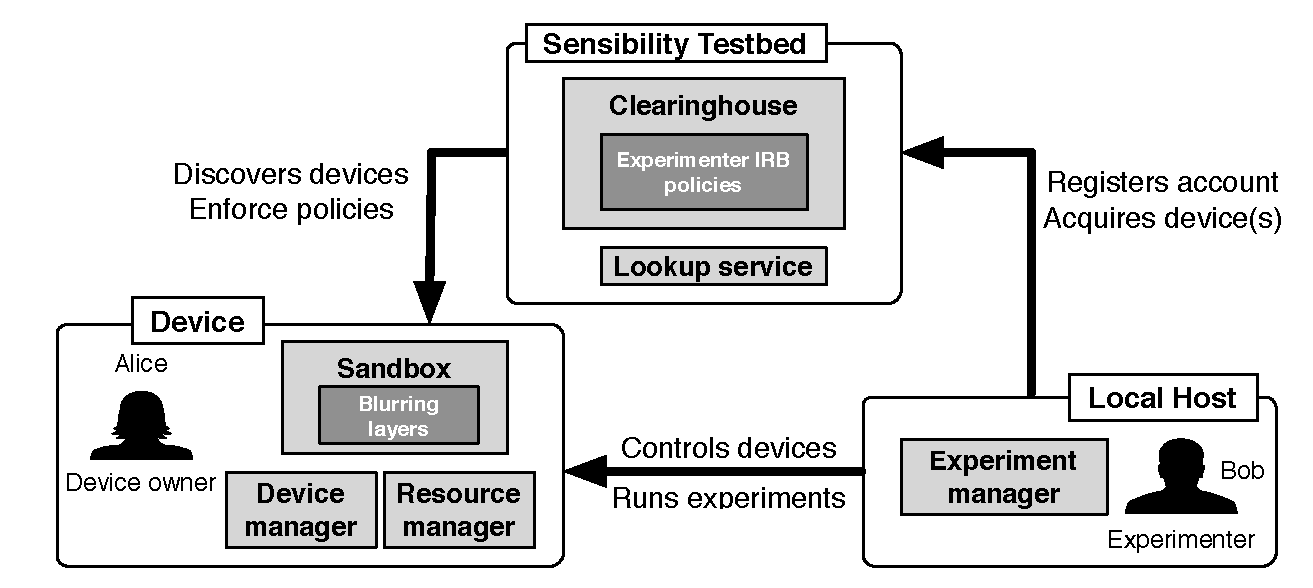
\includegraphics[width=\columnwidth]{figs/arch.pdf}}
%\vspace*{-20pt}
\caption{\small Sensibility Testbed architecture. \label{fig-arch}}
\end{figure}

This section addresses how these elements interact to
enable safe experimentation on mobile devices. First, 
a researcher needs to provide his institute's 
IRB policies for accessing devices to the clearinghouse 
server (Section~\ref{sec-ch}). \yanyan{need a screenshot} 
%These policies restrict what and how data can be accessed by the 
%researcher. 
The clearinghouse server helps the researcher acquire and manage
devices, and codifies the policies specified by the
researcher's IRB. 
%into data blurring layers that are enforced on
%mobile devices. Such a process can protect device
%owners' personal information. 
After obtaining remote devices, researchers can perform
experiments directly on the devices, using the credentials assigned by
the clearinghouse. Researchers' code runs in a sandbox 
that isolates the code from the rest of the device
host system (Section~\ref{sec-repy}). To control the execution of 
code, the researcher uses his own desktop or laptop computer to manage the 
experiments via an experiment manager. This tool can deploy 
and run experiments in sandboxes on remote devices that are 
acquired through the clearinghouse (Section~\ref{sec-emt}).

%\subsubsection{Enforcing IRB Approved Policies}


\subsection{Testbed Components}\label{sec-component}

The components of the Sensibility Testbed are shown in Figure~\ref{fig-arch}.
Each is critical to the operation of the testbed. 
In this section, we describe the function of each component: the
software running on a mobile device, the clearinghouse~\cite{ch}, 
and experiment manager.

To demonstrate how these components interact with each other, we assume 
that a smartphone owner, Alice, participates in the testbed; a researcher, Bob, 
runs code on Sensibility Testbed using Alice's smartphone, among other
devices discovered. Specifically, Bob wants to know the cellular service
quality in major cities. As such, he needs location information
of individual devices, their cellular service provider, network
type (3G, 4G, LTE, etc.), and signal strength.

\subsubsection{Device Software}\label{sec-repy}

%In Sensibility Testbed, all experiments execute in a secure 
%sandbox on the end devices.
%Experimenters' code executes in a sandbox that isolates the 
%experiment code from the device host system. 
Sensibility Testbed uses a sandbox called Repy (Restricted 
Python)\footnote{\scriptsize This is the 
same security-reviewed sandbox~\cite{cappos2010retaining} used in
our prior work, the Seattle testbed~\cite{seattle}. This sandbox
mitigates the impact of bugs in experimenter code.}, which 
provides security isolation and performance isolation on mobile devices.
%Instead of developing full-fledged Android apps, all 
%experiments in Sensibility Testbed are written in a language
%similar to Python, and run in a secure %Python-based
Experimenters use a Python-like programming interface~\cite{repyv2}
to write experiment code, upload the code and execute it in the
sandbox on remote devices. The programming interface includes functions for networking, 
file system access, threading, locking, logging, and so on. To access sensors, 
the sandbox also has a set of sensor functions~\cite{sensors}. 
Details about implementing the Repy sandbox for mobile 
devices are described in Section~\ref{sec-repy-ext}.

%However, the current Repy sandbox does not include calls to access sensors. 
%%To obtain the sensor data, we need to extend the sandbox. 
%The extended Repy sandbox that allows sensor access  
%will be described in Section~\ref{sec-repy-ext}.
Furthermore, the Repy sandbox allows us to change the 
behavior of its programming interface, and control the 
data gathered from the device to adapt to any IRB proscribed limits. 
%For  an experiment
%that involves GPS location, a privacy policy might restrict the
%level of data granularity available to the experiment. For example, it can
%obfuscate GPS location such that it only identifies the center
%of the city that the device is located in, rather than the exact
%location. Using the same technique, 
To illustrate, the IP address of a device may be anonymized, 
the frequency to access GPS location can be constrained, and 
access to cameras can be disabled. 
%Such privacy protection is a contribution of Sensibility Testbed, 
%which does not exist in any prior work. 
The details of policy implementation are presented in 
Section~\ref{sec-layer} and \ref{sec-nanny}.

\textbf{Usage scenario 1: Smartphone owner volunteers as a testbed participant.}
To install Repy and other software on a device, the owner Alice downloads 
our Sensibility Testbed app from the Google Play Store~\cite{sensibility-app}.
The app displays a consent form, \yanyan{cite link} containing the testbed's 
general usage policy. Alice reviews and must agree to this 
policy before installation. If Alice gives her consent, her device will be 
installed with the Repy sandbox, the native Android code to 
start or stop the sandbox, and an interface to communicate with the testbed 
infrastructure (particularly the clearinghouse, described below). 
By agreeing to our general usage policy, different device 
owners of different ages, from different countries, with different
background need only to opt into our testbed as 
volunteers \textit{once}, at the time of app installation. As a result, an 
experimenter like Bob who wants to conduct a research experiment 
%requests devices through our clearinghouse, which assigns 
%them devices from a set of available resources. As a result, 
%the researcher
does not need to get consent from each subject for each individual
experiment. The testbed thus greatly simplifies the process for both the 
device owners and experimenters. 

Once the app is started, Alice's device can be
discovered by the clearinghouse. Her device periodically contacts 
a lookup service to advertise itself to Sensibility Testbed. 
A lookup service is a distributed key-value store, such as a 
distributed hash table (DHT)~\cite{dht}, that 
allows one to retrieve values associated with keys and to associate 
keys with values. Through the app interface, Alice may uninstall, or 
choose to opt out of individual experiments.

\subsubsection{Clearinghouse}\label{sec-ch}
The clearinghouse~\cite{ch} is a testbed server that keeps 
track of devices and mediates experimenter access to the 
available devices. It allows experimenters to register 
accounts and share access to a common pool of devices.
The clearinghouse does so by looking up available devices, and assigning
them to a researcher's experiment account upon request. 
Its key role is to facilitate device sharing, 
which relieves individual experimenters from repeatedly 
recruiting devices for each experiment.

Note that in Sensibility Testbed, there are two types of keys. A device
owner has an \textit{identification key} to identify the app installed on a 
device. An experimenter has a pair of public/private \textit{authentication 
keys} to authenticate the experimenter with the clearinghouse and 
the set of devices that he has access to.

\textbf{Usage scenario 2: Clearinghouse tracks devices.}
To keep track of Alice's device, the
clearinghouse periodically queries the lookup service to
discover any new devices. Once Alice's device is discovered, the
clearinghouse obtains its \textit{identification key} \path{key.alice} generated
during installation, and stores this key. 
%clearinghouse uses a database that stores her device's unique
%identification key, \path{key.alice}, generated during installation. 
This key is not associated with Alice's or her
device's identity, but only the app's installation on the device. If
Alice uninstalls the Sensibility app, \path{key.alice} is
deleted at the clearinghouse, which effectively unlinks
her device from any metadata stored on the clearinghouse.

%The clearinghouse
%plays an intermediate role between the experimenter and 
%the device owner.
%As described in Section~\ref{sec-overview}, when an 
%experimenter registers at the clearinghouse, he
%needs to provide his IRB policies. These policies ensure that
%the researcher cannot conduct experiments to access data that
%extend beyond the experiment policy. The clearinghouse 
%translates and codifies each policy, and instructs the 
%sandboxes on remote devices to implement these policies. 
%When experiment code is running in the sandbox, the 
%policies will be applied to restrict %the precision of sensor 
%%data or the frequency to access 
%sensor access. 
\textbf{Usage scenario 3: Researcher registers experiment and provides IRB policies.}
To run code on Sensibility Testbed, researcher Bob first needs to 
provide a set of detailed IRB policies from his institution. 
%In order to obtain an IRB approval, a researcher first 
To do this, Bob fills out an experiment
registration form \yanyan{cite url or show screenshot} at the 
clearinghouse. The clearinghouse registration page shows 
a list of sensors accessible through our programming interface, and 
each of their possible accuracy 
and access frequency. In this case, Bob specifies that 
%what data can be accessed by a research experiment, at which 
%granularity or frequency such data can be accessed, how data 
%should be securely stored, and so on. \yanyan{cite register 
%experiment website url.}
his experiment can (1) read location information
from devices at the granularity of a city, (2) read accurate
cellular signal strength and network type, as well as
%but not allow access to information about 
cell IDs, and (3) get location and
cellular network data updates every 10 minutes. 
%Bob submits an
%experiment description for these requirements, which the
%clearinghouse will codify into policies that are later enforced
%on remote mobile devices (Section~\ref{sec-ch}).
%Bob then uses this form, along with other forms downloaded 
%from the clearinghouse, to apply for IRB approval at his institution.
%
Aftering filling out this form, Bob downloads the experiment description 
he provided, the detailed information about Sensibility Testbed and 
several relevant forms, such as 
those addressing consent, terms of participation (for device owners) 
and terms of usage (for the researcher), and so on. \yanyan{cite our docs}  
Bob then uses these forms as a template to complete the IRB registration 
with his institution. These forms serve as a set of reference documents 
to make it easier for researchers like Bob to 
file the necessary IRB paperwork with their institutions.

After the application is submitted, Bob's IRB may disagree with 
his initial experiment requirements. For example, Bob's IRB disagrees 
that his experiment should access cell IDs in cellular networks, but 
approves the other policies. 
%Bob wants to access cell 
%IDs in cellular networks, but his IRB disallows such data access. Bob then
In this case, Bob will revise the experiment requirements, refile the paperwork, 
and obtain IRB approval. Bob then submits the revised experiment 
registration form and his IRB approval to the clearinghouse.

Finally, the clearinghouse
parses Bob's registration form, extracts each data accuracy and access 
frequency approved by Bob's IRB, and assigns an experiment 
account to Bob. Once his account is activated, Bob obtains his 
\textit{authentication keys} assigned by the 
clearinghouse. These keys are to authenticate Bob with the 
clearinghouse and the set of devices that he has access to.
%\path{bob.public} and \path{bob.private}.
Next, Bob can request a number of devices from the 
clearinghouse (Section~\ref{sec-emt}). The clearinghouse has a default set of blurring layers 
for accuracy and access frequency for each sensor. Once Bob requests 
devices, the clearinghouse supplies the extracted data from the 
researcher's registration form as input parameters to
the blurring layers that will be instantiated on the requested devices. 
The poicies are easily customizable. Details about
how each policy is implemented will be introduced in Section~\ref{sec-policy}.


This Sensibility Testbed
clearinghouse protocol for research plays a central role in
easing the device recruitment and experiment setup for experimenters, 
and ensures the enforcement
of privacy policies\footnote{\scriptsize The Sensibility Testbed Clearinghouse
protocol for research with human subjects has been approved by
the IRB at New York University (IRB \# 15-10751).}. 


\subsubsection{Experiment Manager}\label{sec-emt}

To run code remotely on mobile devices, a researcher will use an
experiment manager dowloaded to his own computer 
%which contains Bob's private key, \path{key.bob-priv}, 
to access the sandboxes on the remote devices assigned by the clearinghouse. 
This experiment manager provides a light-weight command line 
console~\cite{demo-kit} that allows direct access from the 
experimenter's local machine to a set of remote devices. 

\textbf{Usage scenario 4: Researcher acquires device(s) and runs an experiment.}
%\label{sec-acquire-run}
%The above clearinghouse protocol ensures the enforcement of data
%access policies. Additionally, 
To perform an experiment, Bob needs some devices under his 
experiment account. 
%Recall that a testbed-specific key, \path{key.sensibility}, is distributed
%with the Sensibility Testbed app downloaded and installed by device
%owners (Section~\ref{sec-owner-participate}). 
%
%\yanyan{Albert thinks this is too much detail.}
%At this moment,  Bob has obtained an account with the clearinghouse.
%and is assigned a pair of public and 
%private keys, \path{key.bob-pub} and \path{key.bob-priv}, by the
%clearinghouse. 
When Bob requests a device, the clearinghouse
happens to find that Alice's device is available from the lookup service
(usage scenario 2). The clearinghouse then 
%adds Bob's public key, \path{key.bob-pub}, to
%the sandbox on Alice's device. This indicates that Bob is
%authorized to use this sandbox on Alice's device, and 
assigns Alice's device to Bob's experiment account by placing Bob's
public key on Alice's device. It then instructs 
the sandbox on Alice's device to add Bob's policies by preloading
a set of blurring layer code. At this point, Bob can access Alice's 
device through the experiment manager, just like using \texttt{ssh}.
%Bob writes his experiment 
%code in the Python-like language supported by our secure sandbox.
%The following is a snipet of code that gets location coordinates 
%from a device:

Next, Bob uploads his code to Alice's device and 
runs his experiment. When he accesses the device through
the experiment manager, the sandbox on Alice's device 
applies the data access policies loaded by the clearinghouse: For 
policy (1), the sandbox blurs the location
information returned from Alice's phone down to the coordinates
of the nearest city; for policy (2), the sandbox blocks the
access to cell IDs; for policy (3), the sandbox limits the rate
of GPS location and cellular network queries from Bob's
experiment to one in every 10 minutes.

The clearinghouse has no involvement after Bob deploys 
his experiment and runs the code, and it does not store any
data on Bob's behalf. After collecting the data he needs, Bob 
can use the experiment manager to download data from the remote devices. 
Alternatively, he can set up his own server to store all the data\footnote{\scriptsize
If an experimenter stores data on his own server, he must use protective
measures to ensure that the data sent from the mobile devices is
properly encrypted, and the server storage cannot be tampered
with by any other parties. This is enforced by requiring the experimenter to register
his server by providing its certificate and URL to our
clearinghouse. Following receipt of this data, the clearinghouse will instruct the devices
accessible to the experimenter that all the sensor data collected should be
sent to this server. The sandboxes on these devices will issue
\texttt{HTTPS POST} using the server's certificate, and send encrypted
data to the experimenter's server.}, or use a data 
store service we provide (a service called Sensevis~\cite{sensevis}, 
not shown in Figure~\ref{fig-arch}). After the data is collected, how to store
the data securely is mandated by Bob's IRB.

\smallskip
In summary, 
%Prior to running an experiment on Sensibility Testbed, a
%experimenter first fills out a form in plain text to describe the
%purpose of the research experiment. This experiment description
%is created at the Sensibility Testbed clearinghouse
%where the researcher indicates the type of data to be collected,
%how that data will be used and stored, and so on. 
%
%Once this information is collected from the researcher, the
%clearinghouse automatically generates a set of blurring layers
%that implements the experiment policy (Section~\ref{sec-policy}). In
%Sensibility Testbed, researchers can collect data from the
%sensors on the device, such as GPS, Bluetooth, battery
%information, accelerometer, light, and orientation,
%etc. The blurring layers we provide consist of
%data access restrictions, created in accordance with
%researcher's experiment description, by using the Sensibility
%Testbed's sandboxing technique 
%(Section~\ref{sec-repy})~\cite{cappos2010retaining}. These restrictions ensure that
%the researcher cannot conduct experiments to access data that
%extend beyond the experiment policy. 
%
%This Sensibility Testbed
%clearinghouse protocol for research plays a central role in
%easing the approval process of IRB, and ensures the enforcement
%of privacy policy\footnote{The Sensibility Testbed Clearinghouse
%protocol for research with human subjects has been approved by
%the IRB at New York University. \yanyan{might need a link to
%your approval letter or ref number}}. 
using Sensibility Testbed, device owners' privacy is protected
from any inadvertent or malicious attempt, and researchers 
are able to go through a streamlined process of device 
recruitment and experiment setup.

%the device owners do not need to give consents 
%multiple times, to each project of each researcher. 
%In the following, we present several usage scenarios to
%demonstrate how device owners opt in as volunteers, and how
%researchers do experiments on devices without compromising device
%owners' privacy.

%\subsection{Testbed Usage Scenarios}\label{sec-scenario}


\subsection{Sensibility Testbed's Default Policies}\label{sec-irb-policies}

%In the domain of IRB, Alice and Bob are the participating subject, and 
%a researcher who conducts a research study on the subject, respectively.
%
%
%\textbf{Sensibility Testbed's default policies.}

\begin{table}
\scriptsize
\centering

\bgroup
\def\arraystretch{1.15}% % for table padding
\begin{tabular}{|l|c|c|c|}
\hline
\multirow{2}{*}{\bf Sensor} & 
\multicolumn{3}{c|}{\bf Default policy} \\\cline{2-4}
& {\bf LR} & {\bf MR} & {\bf HR} \\\hline

Battery (plug-in type, level, technology, etc.) & \tickmark &  & \\ \hline
Bluetooth (local name, scan mode, etc.) & & \tickmark & \\ \hline

\multirow{2}{5.5cm}{Cellular network (cell ID, area code, country code, 
operator name, etc.)} & & \multirow{2}{*}{\tickmark} & \\ 
& & & \\ \hline

Location (latitude, longitude, altitude, speed, etc.) & & \tickmark & \\ \hline
Settings (screen brightness, ringer volume, etc.) & & \tickmark & \\ \hline

\multirow{2}{5.5cm}{Motion sensors (accelerometer, 
gyroscope, magnetometer, orientation , etc.)} & & \multirow{2}{*}{\tickmark} & \\ 
& & & \\ \hline

\multirow{2}{5.5cm}{WiFi network (information about the 
currently active access point, and WiFi scan result)} & & \multirow{2}{*}{\tickmark} & \\ 
& & & \\ \hline 

%Start/stop activities & & & \xmark \\ \hline 
%Running applications & & & \xmark \\ \hline 
Camera (take pictures, record videos) & & & \xmark \\ \hline 
Intent (scan barcode, search, etc.) & & & \xmark \\ \hline 
Address book & & & \xmark \\ \hline 
Microphone (voice record) & & & \xmark \\ \hline 
SMS (send/receive messages, delete messages) & & & \xmark \\ \hline 

\end{tabular}
\egroup

\caption{\small Sensibility Testbed's default policies for sensors. LR/MR/HR
stands for low/moderate/high risk, respectively. Only sensors that have low to 
moderate risks are allowed (\tickmark). Sensors that are highly risky are 
disabled by default (\xmark).}
\label{tab:default}
%\vspace{-10pt}
\end{table}


Note that Bob cannot request complete access to all sensors 
even if his IRB approves such a policy. The Sensibility Testbed's
own IRB designates a set of default policies to access sensors in a
way that is low to moderate risk. 
%and for which access can be pre-approved with the
%researcher's local IRB. 
Only those sensors listed on our project 
wiki page~\cite{sensor-api} are accessible to a researcher. 
A summary of these sensors is listed in Table~\ref{tab:default}, 
where each sensor is categorized as of low, moderate or high 
privacy risk.

The list of sensors that Sensibility Testbed provides are of moderate 
to low privacy risks (marked by \tickmark), and the testbed further provides policy enforcement
(Section~\ref{sec-policy}) to protect all the sensor data. Sensors 
such as cameras and microphones that are deemed sensitive are not 
exposed to experiment code (marked by \xmark). This is motivated by the Android system, 
where permissions are categorized into different protection levels~\cite{level}:
\textit{normal} permissions are automatically granted to the apps, 
\textit{dangerous} permissions are given based upon the 
user's consent, and so on. Furthermore, 
%we divide sensors into different risk levels, as shown 
%in Table~\ref{tab:default}. 
%Sensors with low to moderate risk are 
%allowed and protected by IRB policies. Sensors of high risk are 
%disabled by default. 
we divide sensors into different risk levels by the consequences and 
difficulties of a potential attack. If a microphone is controlled by 
a malicious party, it can be used to intelligently choose data of a 
higher value (e.g., credit card number, password) to record~\cite{zhang2015leave}. On the other 
hand, in order to infer credit card number or password typed on a 
smartphone using motion sensors, an sophisticated algorithm needs to 
be installed on the device and constantly learn about  
the patterns of data generated by accelerometer or gyroscope. In contrast,
using battery information alone is not sufficient to create a fingerprint 
for each device. Different information and mutiple occurrence need to
be pieced together~\cite{battery-priv}. Therefore, 
compared to motion sensors, a microphone is considered of higher risk, 
and battery is of lower risk than both the motion sensors and a microphone.

Although high-risk sensors are disabled, if such access  is critical to the 
study, a different IRB procedure could be followed. 
In this case, the research project has to go through the Sensibility 
Testbed's IRB, in addition to the researcher's IRB. 
\yanyan{if we think this is ok, then we provide specially
designed interface and policy?}
%Depending on the experiment description provided by the 
%researcher, the fields marked with a (*) are the ones that will be blurred.
%
%
As a result, Sensibility Testbed does not
provide unfettered access to all sensors. 
%Access to sensors of
%higher risk, e.g., the policies that request restricted sensor data, 
%or at higher frequencies than our default policies, 
%needs to go through the Sensibility Testbed's IRB,
%in addition to the researcher's IRB. 
The default policies serve as a common denominator to all 
researchers' IRB policies. In most cases, we expect
that researchers need only go through their local IRB to get
the sensor access they need for their experiment. 
